\chapter{Exploration: Contextual and Bayesian bandits,  Thompson sampling}

In the previous chapter, we discussed the multi-armed bandit (MAB) problem, which involves making decisions (pulling arms) in a stateless environment. That is, the agent repeatedly chooses an action without considering any additional information that might influence its decision-making. Each arm has an unknown reward distribution, and the agent's goal is to balance exploration (learning about the rewards of different arms) and exploitation (choosing the arm with the highest expected reward).

However, real-world scenarios often provide more information that can help us make better decisions. For instance, a recommendation system might know a user's preferences, or a robot might observe its environment before acting. This kind of context can guide the decision-making process more effectively than pure exploration of actions.

Contextual bandits extend the MAB framework by introducing a state or context that is available before each decision. This additional information allows the agent to choose actions based not only on past rewards but also on the context of the current situation.

In contextual bandits, the interaction process is as follows:
\newpage
\begin{enumerate}
    \item A random state $x_t$ is sampled from the environment's state distribution $\mu$ \begin{center}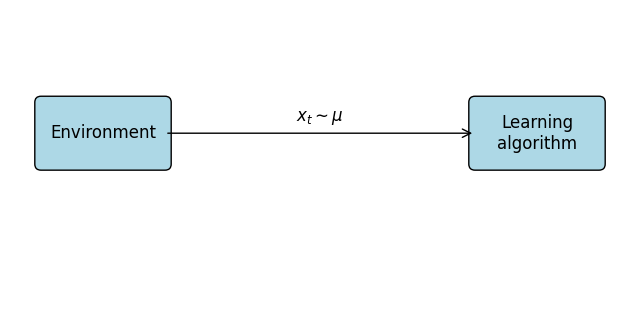
\includegraphics[width = 10cm]{Exploration - Contextual and Bayesian bandits, Thompson sampling/interaction_sampling.png} \end{center}
    \item The learning algorithm processes the state and outputs an action $a_t$ \begin{center}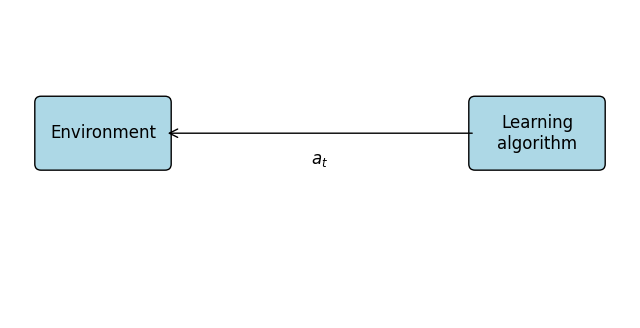
\includegraphics[width = 10cm]{Exploration - Contextual and Bayesian bandits, Thompson sampling/interaction_action.png} \end{center}
    \item After the action, the environment provides a reward $r_t$ indicating the quality of that action. \begin{center}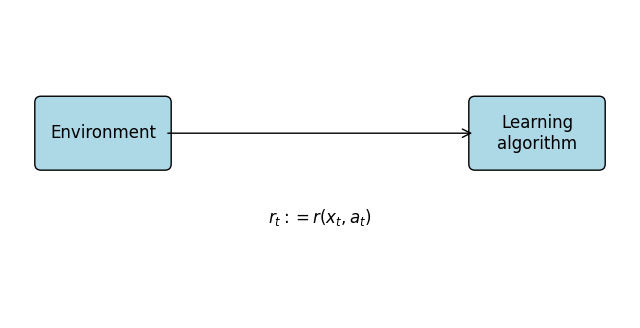
\includegraphics[width = 10cm]{Exploration - Contextual and Bayesian bandits, Thompson sampling/interaction_reward.png} \end{center}
\end{enumerate}

\begin{warningbox}[Warning]
    Contextual bandits are a simplified version of reinforcement learning (RL), where we don't deal with the complexity of state transitions over time. In a standard RL setup, an agent’s actions can change the state of the environment. However, in contextual bandits, the environment resets after each action, and we assume that the states we observe in each round are not influenced by previous actions. This i.i.d. assumption simplifies the analysis by treating each round as independent of the others.
\end{warningbox}

\section{Policy}

In a contextual bandit setting, a policy $\pi$ is a strategy that \textbf{for all states} determines which action to take based on the given context (the state).

A policy maps the current sampled state $x_t$ to an action $a_t$. The policy can be deterministic, meaning that for a given state $x_i$, the policy always selects the same action $a_i = \pi(x_i)$. Alternatively the policy can be stochastic, where given context $x_i$, the action is sampled from a probability distribution over possible actions, $a_i \sim P(a_i | x_i)$

\begin{warningbox}[Warning]
    We assume to work only with deterministic policies for now
\end{warningbox}

\section{Regret}
In the contextual bandit problem, the regret quantifies the difference between the total reward that would have been obtained by always following the optimal policy $\pi*$ and the total reward obtained by following the learned sequence of policies $\pi^t$ over time.

We define the regret as follow:

$$
    R_T = T \mathbb{E}_{x \sim \mu} [r(x, \pi^*(x))] - \sum_{t=0}^{T-1} \mathbb{E}_{x \sim \mu} [r(x, \pi^t(x))]
$$

\begin{tipbox}[Explanation]
    We use expected values because we are dealing with uncertainty and randomness in both the context and the rewards.
\end{tipbox}

\newpage

\section{Explore and commit algorithm}

We can introduce a version of the explore and commit algorithm in the contextual bandit as follows:

\begin{algorithm}
    \caption{Explore \& Commit Algorithm}
    \begin{algorithmic}[1]
        \State \textbf{Input:} Time horizon $T$, exploration phase length $N$
        \State \textbf{Initialize:} Empty set of observations for each action $a \in A$

        \State \textbf{Exploration phase:}
        \For{$t = 0, \dots, N-1$}
        \State Observe state $x_t \sim \mu$
        \State Uniformly sample action $a_t \sim \text{Unif}(A)$
        \State Observe reward $r_t = r(x_t, a_t)$
        \State Store $(x_t, a_t, r_t)$ for all $a \in A$
        \State Build for $x_t$ an unbiased estimate of $\mathbb{E}_{a_t \sim p} \hat{r}[a] = r(x_t, a), \ \forall a \in A$
        \EndFor

        \State \textbf{Compute policy:}
        \State Compute policy $\hat{\pi}$ as:
        \[
            \hat{\pi} = \arg \max_{\pi \in \Pi} \sum_{i=0}^{N-1} \hat{r}(x_i, \pi(x_i))
        \]

        \State \textbf{Commit phase:}
        \For{$t = N, \dots, T-1$}
        \State Observe state $x_t \sim \mu$
        \State Play arm $a_t = \hat{\pi}(x_t)$
        \EndFor
    \end{algorithmic}
\end{algorithm}


\begin{tipbox}[Explanation]
    $\mathbb{E}_{a_t \sim p} \hat{r}[a] $ denotes the average estimated reward $\hat{r}[a]$ over all possible actions $a_t$, assuming that $a_t$ is chosen according to the probability distribution $p$.

    $\hat{r}[a]$ is the estimate of the reward associated with action $a$. It is important to note that we only observe rewards for the action $a_t$ that is actually taken, but we need to estimate the rewards for all possible actions.

    Finally, the term $r(x_t, a)$ is the true reward for taking action $a$ in state $x_t$. In practice, we do not know this value for all actions, so we estimate it using the observed rewards.

    The goal is to ensure that this estimate is unbiased, meaning it does not systematically overestimate or underestimate the true reward. By making the estimate unbiased, the algorithm avoids favoring or penalizing certain actions unfairly, which is critical for making good long-term decisions in the exploration-exploitation trade-off.

\end{tipbox}

When we sample actions uniformly at random, the probability of selecting any action $a \in A$ is constant. Since we're sampling from a uniform distribution over $A$, the probability $p(a_t)$ is simp